%!TEX root = ComputerScienceOne.tex

%Basic I/O - exercises

\section{Exercises}

%\begin{exer}
%Write a program to convert a temperature in degrees Fahrenheit 
%($f$) to degrees Celsius ($c$), using the equation
%  $$c = \frac{5}{9}\Big(f - 32\Big)$$
%\end{exer}

\begin{exer}
Write a program that calculates mileage deduction for income tax using the
standard rate of \$0.575 per mile.  Your program will read in a beginning
and ending odometer reading and calculate the difference and total 
deduction.  Take care that your output is in whole cents.  An example run
of the program may look like the following.

\begin{minted}{text}
INCOME TAX MILEAGE CALCULATOR
Enter beginning odometer reading--> 13505.2
Enter ending odometer reading--> 13810.6
You traveled 305.4 miles.  At $.575 per mile,
your reimbursement is $175.61
\end{minted}
\end{exer}

\begin{exer}
Write a program to compute the total ``cost'' $C$ of a loan.  That is, the total amount of interest paid over
the life of a loan.  To compute this value, use the following formula.
$$C = \frac{p\cdot i \cdot \left(1 + i\right)^{12n}}{(1+i)^{12n} - 1} * 12n - p$$
where
\begin{itemize}
  \item $p$ is the starting principle amount
  \item $i = \frac{r}{12}$ where $r$ is the APR on the interval $[0, 1]$
  \item $n$ is the number of years the loan is to be paid back
\end{itemize}
\end{exer}

\begin{exer}
Write a program to compute the annualized appreciation of an asset (say a house).  The program
should read in a purchase price $p$, a sale price $s$ and compute their difference $d = s - p$ 
(it should support a loss or gain).  Then, it should compute an appreciation rate: $r = \frac{d}{p}$ along
with an (average) \emph{annualized appreciation rate} (that is, what was the appreciation rate in each
year that the asset was held that compounded ):
$$(1 + r)^{\frac{1}{y}}-1$$
Where $y$ is the number of years (possibly fractional) the asset was held (and $r$ is on the 
scale $[0, 1]$).
\end{exer}

\begin{exer}
The annual percentage yield (APY) is a much more accurate measure of the true cost of a 
loan or savings account that compounds interest on a monthly or daily basis.  For a large enough 
number of compounding periods, it can be calculated as:
 $$APY = e^{i} - 1$$
where $i$ is the nominal interest rate ($6\% = 0.06$).  Write a program that prompts the user 
for the nominal interest rate and outputs the APY.
\end{exer}

\begin{exer}
Write a program that calculates the speed of sound ($v$, feet-per-second) in the 
air of a given temperature $T$ (in Fahrenheit). Use the formula,
 $$v = 1086 \sqrt{\frac{5T + 297}{247}}$$
Be sure your program does not lose the fractional part of the quotient
in the formula shown and format the output to three decimal places.
\end{exer}

\begin{exer}
\label{exercise:radiansToDegree}
Write a program to convert from radians to degrees using the formula
  $$deg = \frac{180\cdot rad}{\pi}$$
However, radians are on the scale $[0, 2\pi)$.  After reading input
from the user be sure to do some error checking and give an error
message if their input is invalid.
\end{exer}

\begin{exer}
Write a program to compute the Euclidean Distance between two points, 
$(x_1, y_2)$ and $(x_2, y_2)$ using the formulate:
$$\sqrt{(x_1-x_2)^2+(y_1-y_2)^2}$$
\end{exer}

\begin{exer}
Write a program that will compute the value of $\sin(x)$ using the first 4 terms of 
the Taylor series:
  $$\sin(x) \approx x - \frac{x^3}{3!} + \frac{x^5}{5!} - \frac{x^7}{7!}$$
In addition, your program will compute the \emph{absolute} difference between this 
calculation and a standard implementation of the sine function supported in
your language.  Your program should prompt the user for an
input value $x$ and display the appropriate output.  Your output should looks \emph{something}
like the following.

\begin{minted}{text}
Sine Approximation
===================
Enter x: 1.15
Sine approximation: 0.912754
Sine value:         0.912764
Difference:         0.000010
\end{minted}
\end{exer}

\begin{exer}
Write a program to compute the roots of a quadratic equation:
  $$ax^2 + bx + c = 0$$
using the well-known quadratic formula:
  $$\frac{-b \pm \sqrt{b^2 - 4ac}}{2a}$$
Your program will prompt the user for the values, $a, b, c$ and output each real root.
However, for ``invalid'' input ($a = 0$ or values that would result in complex roots), the
program will instead output a message that informs the user why that the inputs are invalid
(with a specific reason).
\end{exer}

\begin{exer}
One of Ohm's laws can be used to calculate the amount of \emph{power} 
in Watts (the rate of energy conversion; 1 joule per second) in terms of Amps (a measure of current, 1 amp = $6.241 \times 10^{18}$ 
electrons per second) and Ohms (a measure of electrical resistance).  Specifically:
  $$W = A^2 \cdot O$$
Develop a simple program to read in two of the terms from the user and output the third.
\end{exer}

\begin{exer}
Ohm's Law models the current through a conductor as follows:
 $$I = \frac{V}{R}$$
where $V$ is the voltage (in volts), $R$ is the resistance (in Ohms) and $I$ is the
current (in amps).  Write a program that, given two of these values computes the
third using Ohm's Law.

The program should work as follows: it prompts the user for units of the first value: the user
should be prompted to enter \texttt{V}, \texttt{R}, or \texttt{I} and should then be
prompted for the value.  It should then prompt for the second unit (same options) and then
the value.  The program will then output the third value depending on the input.  An example
run of the program:

\begin{minted}{text}
Current Calculator
==============
Enter the first unit type (V, R, I): V
Enter the voltage: 25.75
Enter the second unit type (V, R, I): I
Enter the current: 72
The corresponding resistance is 0.358 Ohms
\end{minted}
\end{exer}

\begin{exer}
Consider the following linear system of equations in two unknowns:
$$\begin{array}{rcl}
  ax + by & = & c \\
  dx + ey & = & f 
\end{array}$$
Write a program that prompts the user for the coefficients in such a system (prompt for $a, b, c, d, e, f$).  Then 
output a solution to the system (the values for $x, y$).  Take care to handle situations in which
the system is \emph{inconsistent}.
\end{exer}

\begin{exer}
The surface area of a sphere of radius $r$ is
  $$4\pi r^2$$
and the volume of a sphere with radius $r$ is 
  $$\frac{4}{3}\pi r^3$$
Write a program that prompts the user for a radius $r$ and outputs the surface area and volume of 
the corresponding sphere.  If the radius entered is invalid, print an error message and exit.  Your
output should look something like the following.

\begin{minted}{text}
Sphere Statistics
=================
Enter radius r: 2.5
area: 78.539816
volume: 65.449847
\end{minted}
\end{exer}

\begin{exer}
\label{exercise:basics:airDistance}
Write a program that prompts for the latitude and longitude of two locations (an origin and a 
destination) on the globe.  These numbers are in the range $[-180, 180]$ (negative values 
correspond to the western and southern hemispheres).  Your program should then compute 
the air distance between the two points using the Spherical Law of Cosines.  In particular, 
the distance $d$ is
 $$d = \arccos{(\sin(\varphi_1) \sin(\varphi_2) + \cos(\varphi_1) \cos(\varphi_2) \cos(\Delta) )} \cdot R$$
\begin{itemize}
  \item $\varphi_1$ is the latitude of location $A$, $\varphi_2$ is the latitude of location $B$
  \item $\Delta$ is the difference between location $B$'s longitude and location $A$'s longitude
  \item $R$ is the (average) radius of the earth, 6,371 kilometers
\end{itemize}
Note: the formula above assumes that latitude and longitude are measured in radians $r$, $-\pi \leq r \leq \pi$.  
See Exercise \ref{exercise:radiansToDegree} for how to convert between them.  Your program output should 
look something like the following.  

\begin{minted}{text}
City Distance
========================
Enter latitude of origin: 41.9483
Enter longitude of origin: -87.6556
Enter latitude of destination: 40.8206
Enter longitude of destination: -96.7056
Air distance is 764.990931
\end{minted}

\end{exer}

\begin{exer}
Write a program that prompts the user to enter in a number of days.  Your program should
then compute the number of years, weeks, and days that number represents.  For this 
exercise, ignore leap years (thus all years are 365 days). Your output should look something 
like the following.

\begin{minted}{text}
Day Converter
=============
Enter number of days: 1000
That is 
  2 years
  38 weeks
  4 days
\end{minted}
\end{exer}

\begin{exer}
The derivative of a function $f(x)$ can be estimated using the difference function:
  $$f'(x) \approx \frac{f(x+\Delta x) - f(x)}{\Delta x}$$
That is, this gives us an estimate of the slope of the tangent line at the point $x$.  
Write a program that prompts the user for an $x$ value and a $\Delta x$ value and 
outputs the value of the difference function for all three of the following functions:
  $$\begin{array}{rcl}
  	f(x) & = & x^2 \\
	f(x) & = & \sin(x) \\
	f(x) & = & \ln(x)
    \end{array}$$
Your output should looks something like the following.

\begin{minted}{text}
Derivative Approximation
===================
Enter x: 2
Enter delta-x: 0.1
(x^2)'  ~= 4.100000
sin'(x) ~= -0.460881
ln'x(x) ~= 0.487902
\end{minted}

In addition, your program should check for invalid inputs: $\Delta x$ cannot be zero, and $\ln(x)$ is undefined
for $x \leq 0$.  If given invalid inputs, appropriate error message(s) should be output instead.
\end{exer}

\begin{exer}
Write a program that prompts the user to enter two points in the plane, $(x_1, y_1)$ 
and $(x_2, y_2)$ which define a line segment $\ell$.  Your program should then compute 
and output an equation for the perpendicular line intersecting the \emph{midpoint} of $\ell$.  
You should take care that invalid inputs (horizontal or vertical lines) are handled appropriately.
An example run of your program would look something like the following.

\begin{minted}{text}
Perpendicular Line
====================
Enter x1: 2.5
Enter y1: 10
Enter x2: 3.5
Enter y2: 11
Original Line: 
  y = 1.0000 x + 7.5000
Perpendicular Line: 
  y = -1.0000 x + 13.5000
\end{minted}
\end{exer}

\begin{exer}
Write a program that computes the total for a bill.  The program should prompt the user for a 
sub-total.  It should then prompt whether or not the customer is entitled to an employee discount (of 15\%) by 
having them enter 1 for yes, 2 for no.  It should then compute the new sub-total and apply a 7.35\% sales tax, and
print the receipt details along with the grand total.  Take care that you properly round each operation.

An example run of the program should look something like the following.

\begin{minted}{text}
Please enter a sub-total: 100
Apply employee discount (1=yes, 2=no)? 1

Receipt
========================
Sub-Total   $  100.00
Discount    $   15.00
Taxes       $    6.25
Total       $   91.25
\end{minted}
\end{exer}


\begin{exer}
The ROI (Return On Investment) is computed by the following formula:
  $$\textrm{ROI} = \frac{\textrm{Gain from Investment} - \textrm{Cost of Investment}}{\textrm{Cost of Investment}}$$
Write a program that prompts the user to enter the cost and gain 
(how much it was sold for) from an investment and computes and
outputs the ROI.  For example, if the user enters \$100,000 and
\$120,000 respectively, the output look similar to the following.

\begin{minted}{text}
Cost of Investment: $100000.00
Gain of Investment: $120000.00
Return on Investment: 20.00%
\end{minted}
\end{exer}

\begin{exer}
Write a program to compute the real cost of driving.  Gas
mileage (in the US) is usually measured in miles per gallon
but the real cost should be measured in how much it costs 
to drive a mile, that is, dollars per mile.  Write a program to 
assist a user in figuring out the real cost of driving.  Prompt 
the user for the following inputs.
\begin{itemize}
  \item Beginning odometer reading
  \item Ending odometer reading
  \item Number of gallons it took to fill the tank
  \item Cost of gas in dollars per gallon
\end{itemize}
For example, if the user enters 50,125, 50,430, 10 (gallons), 
and \$3.25 (per gallon), then your output should be something 
like the following.

\begin{minted}{text}
Miles driven: 305
Miles per gallon: 30.50
Cost per mile: $0.11 
\end{minted}
\end{exer}

\begin{exer}
A \emph{bearing} can be measured in degrees on the scale 
of $[0, 360)$ with $0^\circ$ being due north, $90^\circ$ due 
east, etc.  The (initial) directional bearing from location $A$ 
to location $B$ can be computed using the following formula.
$$\theta = \mathrm{atan2}\big(\sin(\Delta) \cdot \cos(\varphi_2), \, \cos(\varphi_1)\cdot\sin(\varphi_2) - \sin(\varphi_1)\cdot \cos(\varphi_2) \cos(\Delta)\big)$$
Where
\begin{itemize}
  \item $\varphi_1$ is the latitude of location $A$
  \item $\varphi_2$ is the latitude of location $B$
  \item $\Delta$ is the difference between location $B$'s longitude 
  	and location $A$'s longitude
  \item $\textrm{atan2}$ is the two-argument arctangent function
\end{itemize}
Note: the formula above assumes that latitude and longitude 
are measured in radians $r$, $-\pi < r < \pi$.  To convert from 
degrees $d$ ($-180 < d < 180$) to radians $r$, you can use the 
simple formula:
  $$r = \frac{d}{180} \pi$$
Write a program to prompt a user for a latitude/longitude of two 
locations (an origin and a destination) and computes the directional
bearing (in degrees) from the origin to the destination.  For example, if
the user enters: $40.8206, -96.7056$ ($40.8206^\circ$ N, $96.7056^\circ$ W)
and $41.9483, -87.6556$ ($41.9483^\circ$ N, $87.6556^\circ$ W), your
program should output something like the following.

\begin{minted}{text}
From (40.8206, -96.7056) to (41.9483, -87.6556): 
bearing 77.594671 degrees
\end{minted}
\end{exer}


\begin{exer}
General relativity tells us that time is relative to your velocity.  
As you approach the speed of light ($c = 299,792$ km/s), 
time slows down relative to objects traveling at a slower velocity.  
This \emph{time dilation} is quantified by the Lorentz equation
  $$t' = \frac{t}{\sqrt{1-\frac{v^2}{c^2}}}$$
Where $t$ is the time duration on the traveling space ship and 
$t'$ is the time duration on the (say) Earth.  
  
For example, if we were traveling at 50\% the speed of light 
relative to Earth, one hour in our space ship ($t=1$) would 
correspond to 
  $$t' = \frac{1}{\sqrt{1-(.5)^2}} = 1.1547$$
hours on Earth (about 1 hour, 9.28 minutes).

Write a program that prompts the user for a velocity which represents the
\emph{percentage} $p$ of the speed of light (that is, $p = \frac{v}{c}$) and
a time duration $t$ in hours and outputs the relative time duration on Earth.

For example, if the user enters $0.5$ and $1$ respectively as in our example, it
should output something \emph{like} the following:

\begin{minted}{text}
Traveling at 1 hour(s) in your space ship at
50.00% the speed of light, your friends on
Earth would experience:
1 hour(s)
9.28 minute(s)
\end{minted}

Your output should be able to handle years, weeks, days, hours, and minutes.  So
if the user inputs something like $0.9999$ and $168$, your output should
look something like:

\begin{minted}{text}
Traveling at 168.00 hour(s) in your space ship at
99.99% the speed of light, your friends on 
Earth would experience: 
1 year(s)
18 week(s)
3 day(s)
17 hour(s)
41.46 minute(s)
\end{minted}
\end{exer}

\begin{exer}
Radioactive isotopes decay into other isotopes at a rate that is
measured by a half-life, $H$.  For example, Strontium-90 has a half-life
of 28.79 years.  If you started with 10 kilograms of Strontium-90, 28.79
years later you would have only 5 kilograms (with the remaining 5 kilograms
being Yttrium-90 and Zirconium-90, Strontium-90's decay products).

Given a mass $m$ of an isotope with half-life $H$ we can determine
how much of the isotope remains after $y$ years using the formula,
  $$r = m \cdot \left(\frac{1}{2}\right)^{(y/H)}$$
For example, if we have $m = 10$ kilograms of Strontium-90 with $H = 28.79$, 
after $y = 2$ years we would have 
  $$r = 10 \cdot \left(\frac{1}{2}\right)^{(2/28.79)} = 9.5298$$
kilograms of Strontium-90 left.

Write a program that prompts the user for an amount $m$ (mass, in kilograms) 
of an isotope and its half-life $H$ as well as a number of years $y$ and 
outputs the amount of the isotope remaining after $y$ years.  For the
example above your output should look something like the following.

\begin{minted}{text}
Starting with 10.00kg of an isotope with half-life
28.79 years, after 2.00 years you would have
9.5298 kilograms left.
\end{minted}
\end{exer}

\begin{exer}
In sports, the \emph{magic number} is a number that indicates the
combination of the number of games that a leader in a division must win and/or
the 2nd place team must lose for the leader to clinch the division.  The
magic number can be computed using the following formula:
  $$G + 1 - W_A - L_B$$
where $G$ is the number of games played in the season, $W_A$ is the number
of wins the leader currently has and $L_B$ is the number of losses the 2nd
place team currently has.

Write a program that prompts the user to enter:
\begin{itemize}
  \item $G$, the total number of games in the season
  \item $W_A$ the number of wins of the leading team
  \item $L_A$ the number of losses of the leading team
  \item $W_B$ the number of wins of the second place team
  \item $L_B$ the number of losses of the second place
\end{itemize}
Your program will then output the current win percentages of both teams,
the magic number of the leading team as well as the percentage of the
remaining games that must go in team A's favor to satisfy the magic
number (for this, we will assume A and B do not play each other).

For example, if a user enters the values 162, 96, 58, 93, 62, the output
should look something like the following.

\begin{minted}{text}
Team Wins Loss Perc   Magic Number
A    96   58   62.34% 5 
B    93   62   60.00%
With 15 total games remaining, 33.33% must go in Team A's favor
\end{minted}
\end{exer}

\begin{exer}
The \emph{Doppler Effect} is a change in the observed 
spectral frequency of light when objects in space are moving toward or away
from us.  If the spectral frequency of the object is known, then the
relative velocity can be estimated based on either the blue-shift (for
objects traveling toward the observer) or the red-shift (for objects
traveling away from the observer) of the observed frequency.  

The blue-shift equation to determine velocity is given by 
$$v_b = c\left(\frac{\lambda}{\lambda_b} - 1\right)$$
The red-shift equation to determine velocity is given by
$$v_a = c\left(1 - \frac{\lambda}{\lambda_r}\right)$$
where
\begin{itemize}
  \item $c$ is the speed of light (299,792.458 km/s)
  \item $\lambda$ is the actual spectral line of the object (ex: 
  	hydrogen is 434nm)
  \item $\lambda_r$ is the observed (red-shifted) spectral line and
  	$\lambda_b$ is the observed (blue-shifted) spectral line
\end{itemize}

Write a program that prompts the user to enter which spectral shift they
want to compute (1 for blue-shift, 2 for red-shift).  The program should then
prompt for the spectral line of an object and the observed
(shifted) frequency and output the velocity of the distant object.
For example, if a user enters the values 1 (blue-shifted), 434 (nm) 
and 487 (nm), the output
should look something like the following.

\begin{minted}{text}
Spectral Line: 434nm
Observed Line: 487nm
Relative Velocity: 32626.28 km/s
\end{minted}
\end{exer}

\begin{exer}
Radiometric dating is a technique by which the age of rocks, minerals, 
and other material can be estimated by measuring the proportion of radioactive
isotopes it still has to its decay products.  It can be computed with the
following formula:
 $$D = D_0 + N (e^{\lambda t} - 1)$$
where
\begin{itemize}
  \item $t$ is age of the sample,
  \item $D$ is number of atoms of the daughter isotope in the sample,
  \item $D_0$ is number of atoms of the daughter isotope in the original composition,
  \item $N$ is number of atoms of the parent isotope in the sample 
  \item $\lambda$ is the decay constant of the parent isotope, 
  	$$\lambda = \frac{\ln{2}}{t_{1/2}}$$
	where $t_{1/2}$ is the half-life of the parent isotope (in years).
\end{itemize}
Write a program that prompts the user to enter $D, D_0, N$, and $t_{1/2}$ and 
computes the approximate age of the material, $t$.  

For example, if the user were to enter 150, 50, 300, 28.8 (Strontium-90's half-life)
then the program should output something like the following.

\begin{minted}{text}
The sample appears to be 11.953080 years old.
\end{minted}
\end{exer}

\begin{exer}
Suppose you have two circles each centered at $(0,0)$ and $(d,0)$
with radii of $R, r$ respectively.  These circles may intersect at two points, 
forming an asymmetric ``lens'' as in Figure \ref{fig:circleIntersection}.

The area of this lens can be computed using the following formula:
\begin{gather*}
A = r^2 \cos^{-1}{\left(\frac{d^2+r^2-R^2}{2dr}\right)} + R^2\cos^{-1}{\left(\frac{d^2+R^2-r^2}{2dR}\right)} - \\
\frac{1}{2}\sqrt{(-d+r+R)(d+r-R)(d-r+R)(d+r+R)}
\end{gather*}

Write a program that prompts the user for the two radii and the $x$-offset $d$
and computes the area of this lens.  Your program should handle the special cases 
where the two circles do not intersect and when they intersect at a single point 
(the area is zero).

%\url{http://mathworld.wolfram.com/Circle-CircleIntersection.html}

\begin{figure}[h]
\centering
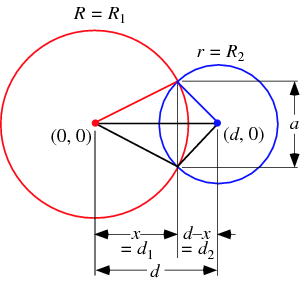
\includegraphics[scale=0.50]{images/circleIntersection}
\caption{Intersection of two circles.}
\label{fig:circleIntersection}
\end{figure}
\end{exer}



